Ранняя и довольно сложная версия того, что мы сегодня называем парашютом описана в работе Леонардо Codex Atlanticus (ок. 1485). Парашют Леонардо состоял из ткани, натянутой на деревянный каркас в форме пирамиды.

\bf{Связанные кольца}

Парашютист Адриан Николас испытал проект Леонардо через 500 лет. Для этого, современная облегченная конструкция соединила парашют Леонардо с телом человека. Мы хотим использовать соединенные кольца, у которых еще предусмотрены крюки для закрепления колец к ткани одежды. Каждое кольцо сделано из гибкого и прочного материала. Кольца легко соединяются вместе, так как каждое кольцо может быть открыто и снова закрыто. Особая конфигурация соединенных колец - это <<цепь>>. <<Цепь>> - это последовательность одного или более колец в которой каждое кольцо соединено только с двумя соседними кольцами, кроме первого и последнего, которые соединены только с одним другим кольцом, как показано ниже. Обратите внимание, что одно кольцо - тоже цепь.

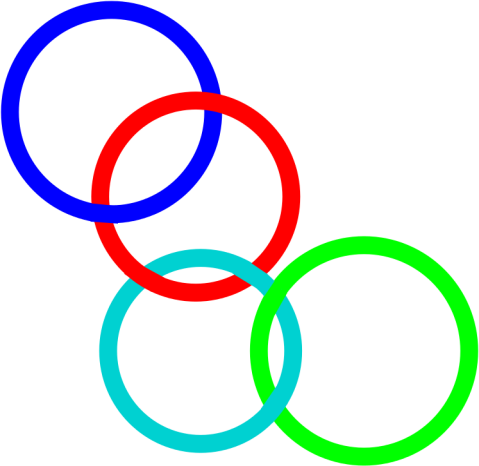
\includegraphics{image_000.png}

Другие конфигурации также возможны, поскольку кольцо может быть соединено с тремя или более другими кольцами. Мы говорим что кольцо <<критическое>>, если после его открытия и удаления, все оставшиеся кольца образуют множество цепей (или не остается других колец). Другими словами, после удаления этого кольца, должны остаться только цепи.

\bf{Пример}

На следующем рисунке представлены семь колец, пронумерованных от $0$ до $6$. Имеется два критических кольца. Одно критическое кольцо - это кольцо номер $2$, так как после его удаления оставшиеся кольца образуют цепи $[1]$, $[0, 5, 3, 4]$ и $[6]$. Другое критическое кольцо с номером $3$, так как после его удаления оставшиеся кольца образуют цепи $[1, 2, 0, 5]$, $[4]$ и $[6]$. Если мы удалим любое другое кольцо, мы не получим множество несвязанных цепей. Например, после удаления кольца номер $5$, хотя мы и имеем цепь $[6]$, но связанные кольца $0, 1, 2, 3$ и $4$ не образуют цепь.

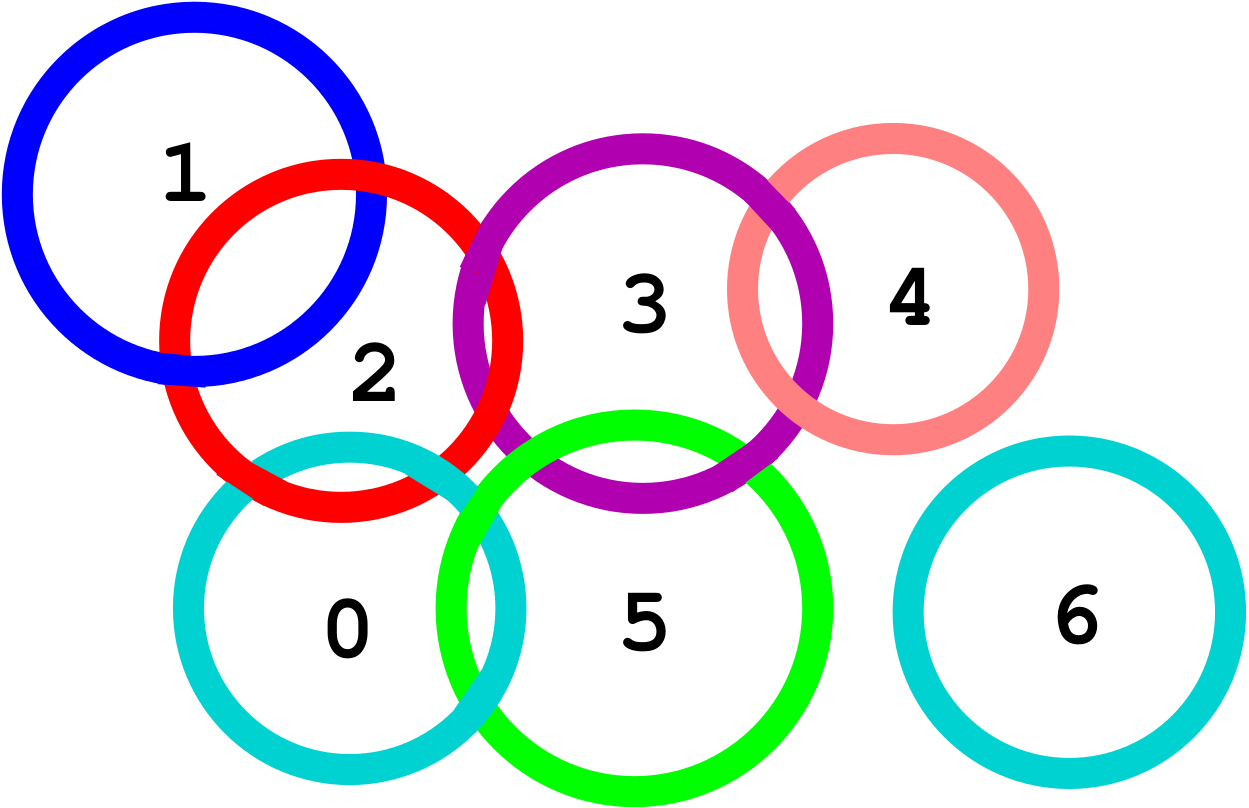
\includegraphics{image_001.png}

\bf{Постановка задачи}

Ваша задача - вычислять количество критических колец в конфигурации, полученной в результате взаимодействия с вашей программой.

В начале, имеется некоторое количество попарно не связанных колец. Затем, кольца связываются вместе. В любой момент времени у вас могут запросить вернуть количество критических колец в текущей конфигурации. А именно, вы должны реализовать три процедуры.

\begin{itemize}
\item \t{Init(N)} --- эта процедура вызывается ровно один раз в начале, чтобы сообщить, что в начальной конфигурации имеется $N$ попарно не связанных колец, пронумерованных от $0$ до $N - 1$ включительно.
\item \t{Link(A, B)} --- два кольца с номерами $A$ и $B$ соединяются. Гарантируется, что $A$ и $B$ различные, и еще не соединены непосредственно; кроме этого, нет дополнительных условий на $A$ и $B$, в частности, нет условий, возникающих из физических ограничений. Ясно, что \t{Link(A, B)} и \t{Link(B, A)} эквивалентны.
\item \t{CountCritical()} --- возвращает количество критических колец для текущей конфигурации связанных колец.
\end{itemize}

Вы должны отправить на проверку ровно один файл, с именем \t{rings.c}, \t{rings.cpp} или \t{rings.pas}. Этот файл должен содержать реализацию подпрограмм используя следующие описания (сигнатуры):

Программы на C/C++:

\begin{itemize}
\item \t{void Init(int N);}
\item \t{void Link(int A, int B);}
\item \t{int CountCritical();}
\end{itemize}

Программы на Pascal:

\begin{itemize}
\item \t{procedure Init(N : LongInt);}
\item \t{procedure Link(A, B : LongInt);}
\item \t{function CountCritical() : LongInt;}
\end{itemize}

Эти подпрограммы должны вести себя как описано выше. Конечно, вы можете реализовывать любые другие подпрограммы для вашего внутреннего использования. Отсылаемые вами на проверку решения не должны никаким образом использовать стандартный поток ввода/вывода или любые другие файлы. 

\bf{Sample grader}

Пример проверяющего модуля (grader) читает входные данные в следующем формате:
\begin{itemize}
\item Строка 1 содержат два числа $N$, $L$;
\item Строки со 2-й по (L+1)-ю содержат:
\begin{itemize}
\item $-1$ для вызова процедуры \t{CountCritical};
\item $A$, $B$ для вызова процедуры \t{Link} с параметрами $A$, $B$.
\end{itemize} \end{itemize}
Пример проверяющего модуля (grader) будет выводить все результаты вызовов функции \t{CountCritical}.